\chapter{绪论}
\section{研究背景}
近年来,一个比较热的人工智能挑战是让计算机参加高考。早在2011年,日本国立情报学研究所(NII)发起了一项名为“东大机器人项目”(Todai Robot Project)的人工智能项目,其最终目的是让此“高考机器人”能够在2021年通过东京大学的入学考试\cite{Fujita}。2015年,国家也启动了863“基于大数据的类人智能关键技术与系统”项目,其目的为攻克高考九门学科中的四门,即语文、数学、地理、历史\cite{Cheng}。本文工作也是对辅助解答地理高考多选题的一些思考尝试,图1所示为2016年上海地理高考多选题:

\begin{figure}[!htb]
	\centering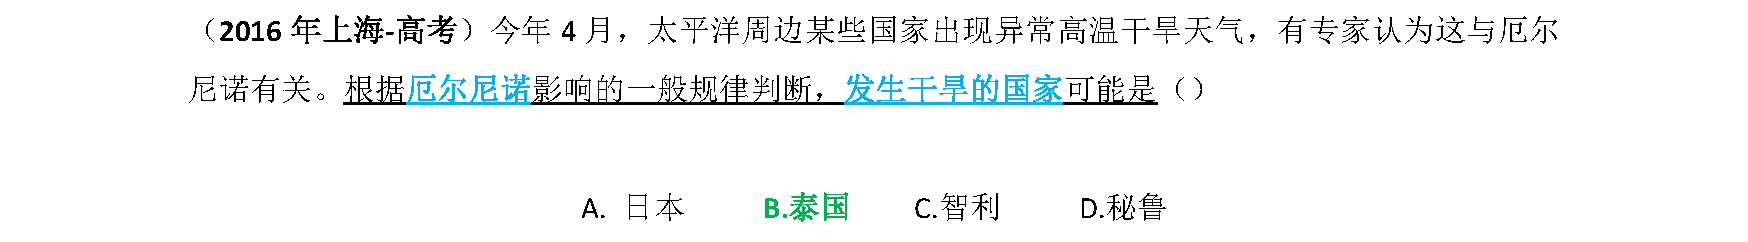
\includegraphics[height=2.2cm]{resource/ex_multi_choice_ques}
	\caption{地理高考多选题举例}
	\label{fig:ex_multi_choice_ques}
\end{figure}

题中划线部分为题目问题,划线部分之前为问题的背景知识介绍。由题可知,问题考察“厄尔尼诺现象会使哪些国家或地区产生干旱现象?”,要解答此问题,计算机必须具备“厄尔尼诺现象”相关的核心知识。如此处需要知道地理知识,厄尔尼诺现象使印度、东南亚、印度尼西亚和澳大利亚产生干旱,然后根据选项中“泰国”属于东南亚,可知此题答案选“泰国”。由上述解题过程可知,解答此类地理问题需要高度结构化的地理知识,并且地理知识表示需包含丰富的语义信息。如此题需要知道“(厄尔尼诺现象,导致干旱的国家,印度、东南亚、印度尼西亚、澳大利亚)”三元组,同时也需要知道“(东南亚,包括,越南、老挝、柬埔寨、缅甸、泰国、马来西亚、新加坡、印度尼西亚、菲律宾、文莱、东帝汶)”,并且还需要知道“东南亚”的类别是一些国家的集合,“泰国”的类别属于东南亚。

鉴于以上分析,解答高考地理题多选题一般可粗粒度分为两步,第一步为匹配求解问题所需的知识库三元组知识,第二步为根据结果三元组作进一步推理得出最终答案。作为辅助解答高考地理选择题中的尝试,本文的工作集中在第一步上,即先构建解答地理高考题所需要的地理核心知识库,再从该知识库中找出最可能回答所求地理问题的三元组知识。

地理解题核心知识库需要高度结构化的知识表示,并且知识需包含丰富的语义信息,如知识类别、关系等。显然,无结构的文本文档以及半结构化的数据(如xml、json格式)表示形式都无法满足要求。在结构化表示领域知识时,本体可以很好对领域知识建模,并且表示出计算机可以处理的带有丰富语义的形式化定义\cite{Hitzler}。前期的地理知识以地理教科书形式存在,地理教科书知识分章节层次描述,计算机是无法处理此种自然语言式的语义关系。因此,需要使用本体对其建模,通过本体中的实体、类别、属性、关系等术语,描述地理中概念(如地球、星球等)的属性信息、类别信息,及各概念之间的相互关系。地理核心知识通过三元组(主、谓、宾形式元祖)形式得以更精炼的表示,地理核心概念层次关系也明显,更适合作进一步的推理。

基于构建的地理核心知识库之上,本文需要构建一个问答系统。给定一个地理问题,系统需返回求解该问题所需的地理知识三元组。目前,基于知识库的问答任务有两个主流的研究方向:基于语义解析\cite{Zettlemoyer0,Cai,BerantCA,Dyer}和基于信息检索\cite{Yao,Bordes1,Dong,Bordes2}。基于语义解析的方法一般先构建一个语义解析器, 然后运用该语义解析器将自然语言问句转换为特定类型的逻辑表达式,如带类型的 lambda 表达式(typed lambda calculus)、 lambda 依存组合语义\cite{Wong,BerantCA,Yih}。基于信息检索的方法通常先从知识库检索一系列候选答案,然后对问句和候选答案进行特征抽取并打分,选出得分最高的结果作为最终答案\cite{Bordes1,Kim}。基于信息检索的方法更简单,实现也更灵活,在开放域知识库Freebase上的问答研究也表明,该方法可以达到与基于语义解析方法相近的 F 值\cite{Dong,Bordes2}。随着深度学习的兴起,神经网络被运用到知识库问答中提升已有模型,基于神经网络的问答模型只需将问题和答案分别表示成地维语义向量,然后通过计算向量相似性,即可获得最相似的候选答案作为最终答案。问句和答案的向量表示是基于神经网络问答模型的一个重要环节,有些研究比较侧重答案表示,如运用候选答案在知识库子图中的重要性\cite{Bordes1}或者答案的类型和上下文\cite{Dong}。这些研究往往使用简单的词袋模型来表示问题,忽视了问题与答案的关联性\cite{Bordes1}。还有研究使用Attention机制根据不同答案的不同注意力方面来表示问题\cite{Zhang},取得了比较好的效果。

分析本文搜集到的地理问题可知,地理问题表达形式多样,无效信息较多,一条地理三元组知识往往可以成为多个地理问题的答案。如三元组——“(季风气候,生产优势,夏季高温多雨、雨热同期)”,可以作为“亚热带季风气候在发展农业生产方面有什么优势” 和“温带季风气候在农业生产方面的显著优势是\_百度知道”这两个问题的答案。虽然两个问题问题表述不一样,但其问题核心均考察“季风气候对生产的优势”,因此相对答案三元组而言它们是等效的。这也说明,在做问答时,单独的将问题和答案表示成向量是不准确的,至少是不能表示出问题和答案之间的关系。因此可以结合Attention机制,在答案向量表示时同时结合对问题的Attention权重,这样可以更合理的表示问题和答案的关系,同时答案中重要信息与问题中重要信息对齐,这样也减弱了问题中无效信息的干扰,使更容易筛选出正确答案。

\section{研究内容}
本文为辅助解答高考地理多选题所做的尝试性工作,本文核心内容为构建地理核心知识库,并从知识库中找出可以回答所求地理问题的知识三元组。因此,本文研究如何使用本体更准确、更精炼地表示地理教科书中的知识,从而构建一个高质量、高可用性的地理本体知识库。同时,本文研究如何更准确表示形式多样的地理问题,从构建的地理知识库中找出可以回答该问题的地理知识三元组,便于解题组作进一步的答案推理,得出问题最终答案。

本文主要研究内容如下:

(1)为解决高度结构化的地理核心知识库缺乏问题,构建了中文地理本体CGeoOnt。CGeoOnt的构建使用OWL本体语言,将地理教材中核心考点的概念属性、核心概念之间的关系形式化表示。然后,运用启发式规则将CGeoOnt与本体Clinga进行融合,采取人工做最终的校验,最后得到更综合的中文地理本体知识库。

(2)为解决地理问题问法多样导致其难以理解问题,使用基于神经注意力机制的双向长短期记忆内存网络知识库问答模型。问答模型不是独立对问题和答案进行词向量表示,而是在充分考虑问题和答案之间的该依赖关系基础上,结合问题对答案进行综合词向量表示。使正确答案三元组与问题关键信息更好的对齐,减弱非关键信息的干扰,从而更易区分相近的答案三元组,使问答模型辨别答案能力更强。

(3)为解决中文地理问答模型在训练和测试中数据集缺失问题,从互联网收集了一个问法多样的中文地理问题集。问题集中的问题知识均来自地理知识库中的核心出题考点,运用百度问题推荐框API和问题搜索API,从互联网获取这些考点的相关地理问题,经机器半自动筛选加人工筛选出其中的有效问题。最后,人工从本文构建的地理知识库中找出能回答这些问题的地理三元组知识,形成最终的问题、答案对数据集。

\section{论文组织}
本文共分为四章,各章的主要内容如下:

(一)第一章介绍相关的研究背景、研究内容以及论文的组织结构。

(二)第二章介绍论文本体构建、知识库问答方法的研究现状以及论文的工作特色。本体构建研究中介绍了主流的人工本体构建方法,并对比几种方法的优缺点;知识库问答方法研究中介绍了两个主流知识库问答——基于语义解析的知识库问答、基于信息检索的知识库问答的流程和优缺点;论文的工作特色中介绍了论文与之前研究的不同之处,以及论文的亮点和创新点。

(三)第三章介绍基于本体的地理知识问答系统的具体实现过程。论文先介绍论文任务和论文系统结构图,然后介绍本文地理本体构建的具体流程,再介绍在构建的地理知识库之上如何构建问答系统用于回答地理问题,最后介绍论文的实验、实验结果和本文地理数据集的构建。

(四)第四章为论文内容的总结,总结本文的工作亮点及不足,并尝试分析未来本文工作可以提升的方向。